\section{Methodology}

\subsection{Threat Models}
To bring the problem to life, we envision a criminal case in our threat model. Bob is a member of an organization embezzling funds through an international shipping company. There are several nefarious tasks which Bob needs to accomplish that he could utilize port 443 exploitations to achieve:
\begin{itemize}
\item Create a \textbf{\textit{covert data channel}} in order to pass along sensitive information like receipts and records while avoiding detection,
\item \textbf{\textit{Communicate anonymously}} with criminal network colleagues to avoid tracing of colleagues, his own geolocation data, and evidence,
\item Establish \textbf{\textit{remote access}} to a machine from endpoints configured to disallow ports like 22,
\item \textbf{\textit{Exfiltrate data}} from a secure source.
\end{itemize}

Alice is an intelligence officer who is monitoring Bob's network data with reasonable suspicion that he is engaged in criminal acts. We will discuss vulnerabilities in Alice's current surveillance framework and how to use \textsc{Forager} to capture and record evidence which can be used to thwart Bob's plans and provide legal support in the case against his embezzlement and fraudulent company.

\subsubsection{Real-Time Monitoring}

In our scenario, Alice possesses a middlebox technology configured to monitor traffic on port 443. It is common for routers or middleboxes to default-ignore traffic on port 443 as there is usually an overwhelming amount of encrypted traffic on this port that is unprocessable~\cite{shane-review-dns-over-http-04}. Attackers who are aware of this strategy may send unencrypted or sensitive information over port 443 in order to avoid surveillance and detection. In criminal operations, these packets could contain significant data. Thus, it is important for middlebox technologies to have a methodology for scanning traffic on port 443 to determine if the data is truly encrypted. If the data is plaintext, it may be directly processed. If it is highly entropic but only compressed, follow-on processing may be capable of decompressing the data. Currently, Alice configures her middlebox to default-ignore traffic on port 443, instead only monitoring port 143 for unencrypted emails. In order to avoid detection by possible surveillance technology, Bob routes his emails through port 443. The receiver is aware of this and listens for this traffic with the IMAP server on the configured port so that it is received. Thus, Bob is able to transmit content in a way that is receivable by the partner as email/IMAP at no additional security overhead but is undetected as Alice's middlebox does not scan port 443.

\subsubsection{Tunnel Tracking}
Tor allows anonymous internet space for pervasive action and may be used to access content which is blocked by firewalls, whether it be censored or illegal activity. While possibly encrypted and encapsulated with layers of addressing in order to anonymize routing, traffic may be synchronized by timing and further analysis in order to determine endpoints~\cite{Simioni2021}. Thus, tracking Tor and being able to further profile Tor usage and content is a useful operation for intelligence and law enforcement. Network Address Translation (NAT) in VPNs prevents traditional ISP tracking. The ability to detect VPN traffic streams and profile their traffic and applications can be additionally useful for network monitoring. In the scenario, Bob is using a VPN to connect to a forum website. He wishes to remain anonymous during this communication. Alice is following Bob's messages, and sees that he regularly communicates using HTTP and IRC protocols on this platform. She configures her middlebox device to promote traffic on several five-tuple-based traffic flows which she knows to be currently associated with Bob's devices. However, dynamic re-configuration of the tunneled network layers causes Alice to lose the data stream and she is no longer able to monitor his messages and record the activity.

\begin{figure} [ht!]
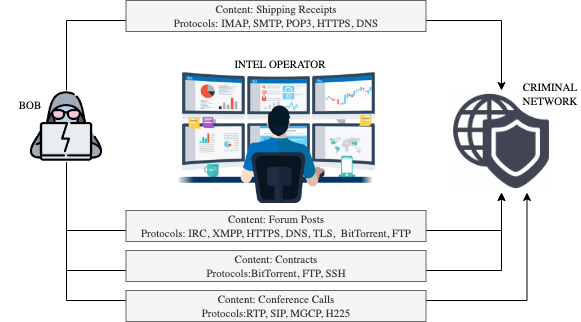
\includegraphics[width=\linewidth]{chapters/7/img/attackscenarios.drawio.png}
\caption{A depiction of intelligence operations intercepting various types of traffic Bob is transmitting in connection to his extended criminal network.}
\label{fig:attacks}
\end{figure}

\subsubsection{Covert Data Channels In}
Domain name security (DNS) has long been exploited by attackers due to many security loopholes and its historical transmission in plaintext. Malicious actors may embed malware or sensitive data into DNS records~\cite{iscx-doh-paper}. This becomes even harder to detect when the tunnel is then encrypted, as is the case with DNS over HTTPS~\cite{rfc8484}. Since its inception, DNS over HTTPS has been adopted by mainstream browsers like Firefox and Chrome to prevent man-in-the-middle attacks and snooping on DNS traffic. While enhancing user privacy, this has contraversely become a field of opportunity for cyber attackers as DNS traffic that is now encrypted may bypass traditional DNS security systems. Thus, the DNS-over-HTTPS (DoH) pipeline can become both a covert channel for malware entering systems as well as data being exfiltrated out. For example, in 2020 the Iranian threat actor group APT34 used DNSExfiltrator2, an open-source DoH tool, to laterally move data to their networks~\cite{quointelligence-apt34}. Malware such as Godlua~\cite{trendmicro-godlua} and PsiXBot~\cite{proofpoint} have also been spotted in the wild along DoH channels. As an example in our scenario, imagine Bob wants to track activity or exfiltrate data from a server in a competitor's private network. In order to record this information, he needs to plant a trojan virus on this server. Using DNS-over-HTTPS as a covert data channel, Bob hosts the trojan on a website and uses social engineering to engage a user to click a link, querying the domain and returning the data which contains the trojan. This malware remains undetected as port 443 traffic is not scanned.

\subsubsection{Covert Data Channels Out}
Many enterprise network environments restrict outbound traffic to ports 80 and 443. Users may re-reroute DNS from the standard port 53 to avoid defeat by firewalls, ISPs, or government or enterprise networks~\cite{shane-review-dns-over-http-04}. Similarly, firewalls can also be bypassed using SSH over port 443. SSH, or secure shell protocol, gives users a method of accessing another computer over an insecure network. While typically transmitted over port 22, many firewalls default to defeating traffic over this port. Instead, they allow traffic over port 443. Packages exist such as \texttt{stunnel} which make SSH tunneling over 443 simple for any internet user~\cite{wong2001stunnel}. Creating a covert data channel over SSH can also be a gateway for cache attacks as it is necessary to transmit or exfiltrate the data when accessed~\cite{Maurice2017HelloFT}. In our scenario, Alice's middlebox technology is monitoring traffic on port 22 (SSH) for secure shell sessions. Bob needs to SSH into a machine and copy over some documents. Instead of relying on traditional channels, Bob has re-routed his SSH connection through port 443, creating a covert data channel. Thus, Alice is missing the mission critical data of the file transfer.

\subsection{System Design}

The \textsc{Forager} system is a highly adaptable traffic profiling multi-tool capable of representing packets in multi-dimensional space through configurable modules. Users can enable up to four different methods of latent representation for the packets. Each of these modules assesses different portions of the packet data with various hidden representation learning approaches. Specifically, \textsc{Alpine} and \textsc{Palm}~\cite{kapoor2022deep} generate one-dimensional locality sensitive hashes which represents single sets of features from the header and payload. \textsc{Maple} and \textsc{Date} generate two-dimensional images and three-dimensional point clouds with clusters, respectively. Votes are provided to the overall framework and used in lookup to generate a classification report. The whole system is depicted in Figure~\ref{fig:forager}.

\begin{figure} [ht!]
\centering
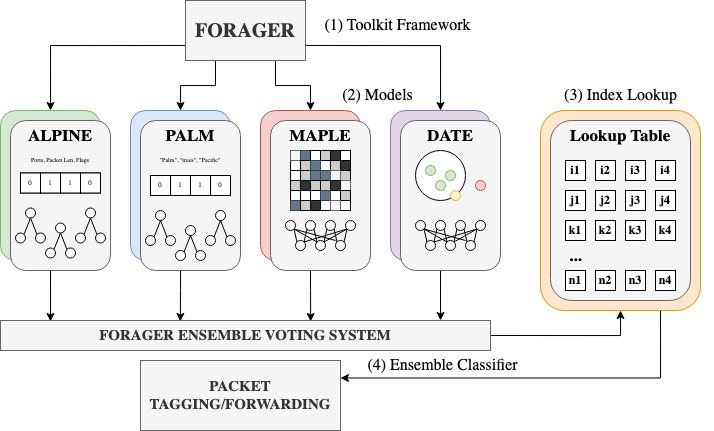
\includegraphics[scale=0.5]{chapters/7/img/forager.png}
\caption{System diagram of \textsc{Forager}.}
\label{fig:forager}
\end{figure}

In the training phase, data is passed in with a label and indexed respective to class. This index is stored in a lookup table inside \textsc{Forager}. Models are enabled or disabled and given a number of votes $m$ per model. This allows the user to more heavily weight one model's opinion over another, further contributing to the flexibility in real deployments. A few additional hyperparameters may be configured for the neural network models such as epochs for training, and data is processed and weights may be saved for later use. In the testing phase, test data is processed in a similar manner and the input passed through the classifier. Forager amalgamates the votes across models and uses its lookup table to return a classification result. In a real packet processing pipeline, we could add this result as part of metadata or an encapsulation header for the packet for downstream processing. The current implementation generates a report of classification results which may be returned to an administrator for further review and possible identification of traffic on non-standard or unexpected ports which could be malicious.

\subsection{Datasets}
To create a pipeline of data representative of a diverse capture on port 443, we utilized several public datasets created by and widely used in the research community for network traffic classification.

\subsubsection{ISCX 2016 VPN-nonVPN Dataset}
We used the UNB ISCX 2016 VPN-nonVPN dataset~\cite{vpn-dataset}. This dataset is a real-world simulation capture created by the Canadian Institute for Cybersecurity (CIC) specifically for encrypted VPN traffic classification~\cite{iscx-vpn-paper}. The traffic was captured using Wireshark and tcpdump and generated using OpenVPN; it contains 28GB of traffic. The packets are a mixture of encrypted and compressed or plaintext traffic. Because these are real-world captures, there are some packets such as ICMP and ARP which are service-level and irrelevant for application and traffic type classification. For this reason, we discard non-TCP/UDP packets as part of the process. Previous work~\cite{deeppacket, Zhou2020, Song2019} in machine learning-based traffic classification has made use of this public dataset and made similar modifications. A breakdown of the dataset is provided in Table~\ref{tab:iscxvpndetails}. The data is divided into the following categories:
\begin{itemize}
    \item \textit{Traffic Type} - There are seven types of traffic: Browsing, File Transfer, Email, Chat, Streaming, VoIP, and P2P.
    \item \textit{Application} - Several of the PCAPs were associated specifically with one application such as Skype or Google Hangouts. The applications we uniquely identify are Pidgin (IAM and ICQ chat), BitTorrent (P2P), Facebook, Skype, Google Hangouts, Spotify, Vimeo, Youtube, Netflix, Thunderbird (Email), and Filezilla (FTP).
\end{itemize}

\begin{table} [ht!]
  \centering
  \begin{tabular}{|p{3cm}|p{8cm}|}
   \hline
   \textbf{Traffic} & \textbf{Content} \\
   \hline
   Browsing & Firefox and Chrome\\
   Email & SMTPS, POP3S and IMAPS\\
   Chat & ICQ, AIM, Skype, Facebook, Hangouts\\
   Streaming & Vimeo, Youtube, Spotify\\
   File Transfer & Skype, FTPS and SFTP using Filezilla\\
   VoIP & Facebook, Skype, Hangouts voice calls\\
   P2P & uTorrent, BitTorrent, Vuze\\
  \hline
  \end{tabular}
  \newline
  \vspace*{0.25 cm}
  \newline
  \begin{tabular}{| c | c | c | c |}
  \hline
   \textbf{Application} & \textbf{Benign} & \textbf{VPN} & \textbf{Tor} \\
   \hline
   AIM chat & 6K & 1.4K & 2K \\
   Email & 50K & 25K & 163K \\
   Facebook & 1837K & 36K & 88K \\
   Filezilla (FTPS) & 312K & 315K & 143K \\
   Filezilla (SFTP) & 629K & 182K & 176K \\
   Gmail & 15K & -- & -- \\
   Chrome & -- & -- & 356K \\
   Hangouts & 1871K & 151K & 1114K \\
   Pidgin (ICQ) & 4K & 7K & 2K \\
   Netflix & 455K & 1433K & -- \\
   SCP & 777K & -- & -- \\
   Skype & 2261K & 1069K & 564K \\
   Spotify & 63K & 193K & 118K \\
   Bittorrent & -- & 133K & -- \\
   VoipBuster & 1017K & 823K & -- \\
   Vimeo & 214K & 591K & 288K \\
   Vuze & -- & -- & 264K \\
   Youtube & 377K & 333K & 261K \\
   \hline
   \end{tabular}
   \caption{ISCX VPN/non-VPN and Tor/non-Tor Datasets}
  \label{tab:iscxvpndetails}
\end{table}

\subsubsection{Tor Datasets}

The Canadian Institute for Cybersecurity similarly created the UNB ISCX 2016 Tor-nonTor~\cite{tor-dataset} dataset which captures data routed over Tor. The traffic was generated using Whonix~\footnote{https://www.whonix.org} and captured using Wireshark and tcpdump; the Tor dataset contains 22GB of traffic. The benign traffic used for comparison in their traffic profiling work~\cite{iscx-tor-paper} is the same from the VPN dataset, establishing a good baseline for our work in combining these two. A gateway was configured to convert non-encapsulated traffic into Tor PCAPs which were then routed to the Tor network. Because Tor is a circuit-oriented network, all traffic from the gateway to the entry node will be routed through the same connection~\cite{iscx-tor-paper} which could cause over-fitting to a particular dataset. In order to better simulate the diversity of network routing methods, we added as another Tor sample PCAPs from Skynet, a Tor-powered botnet with publicly available datasets for research purposes~\cite{skynet}. For a botnet, the advantage of Tor is hidden services. There is no way to trace the original IP address of a hidden server which is published with its .onion pseudo-domain. All botnet traffic is encrypted. The malware which infects the host opens a SOCKS proxy on port 55080 reachable through the .onion domain, and can then run a number of bundled attacks and operations like bitcoin mining, data exfiltration, and DDoS attacks~\cite{skynet}. Thus, we leverage evidence of this botnet implementation as an additional Tor data connection.

\subsubsection{CIRA-CIC-DoHBrw-2020 Dataset}
CIC has also made the CIRA-CIC-DoHBrw-2020 dataset containing DNS-over-HTTPS (DoH) and non-DoH traffic on port 443, with a secondary layer of benign versus malicious DoH traffic~\cite{iscx-doh-paper}. The traffic was generated by querying the top 10K Alexa websites. For non-DoH traffic, an HTTPS request is sent for the website with regular, plaintext DNS. Firefox and Chrome browsers with the configured DNS-over-HTTPS setting were used for benign DoH traffic. For each of the browsers, there were four DNS services used: Cloudflare, AdGuard, Google, and Quad9. Finally, for malicious DoH traffic, tunneling tools dns2tcp, DNSCat2 and Iodine were used to created encrypted TCP covert data channels for transmission. A domain and authoritative name server were established and the DoH tunneling tool used in the client/server interaction. The packet pre-processing we performed on this data was similar to the VPN and Tor dataset processing; a distribution of the data is provided in Table~\ref{tab:dohdataset}.

\subsubsection{EMews SoH Dataset}
SSH is another exploitable protocol for both malware injection and data exfiltration over HTTPS. In 2018, Ricks et al~\cite{Ricks2018ddos} created an SSH over HTTPS (SoH) simulation using the eMews framework and CORE to generate packet traces. The network consists of 1022 nodes, 36 of which incorporate the SSH sessions and the others perform various web-crawling activity for benign comparison. EMews~\footnote{https://mews.sv.cmu.edu/research/emews/} itself is an open-source, large-scale network traffic data generation tool designed to emulate networks employing protocols which require human interaction (ex: starting an SSH connection). Sample counts for this dataset are provided in Table~\ref{tab:sohdataset}.

\begin{table} [ht!]
{
  \centering
  \begin{tabular}{|c|c|c|}
   \hline
   \textbf{Classification} & \textbf{Application} & \textbf{Sample Count} \\
   \hline
   \textit{non-DoH} & Chrome & 542K \\
    & Firefox & 356K \\
   \hline
   \textit{Benign DoH} & Chrome & 3.5K \\
    & Firefox & 16.2K \\
   \hline
   \textit{Malicious DoH} & dns2tcp & 168K \\
   & DNSCat2 & 36K \\
   & Iodine & 47K \\
   \hline
   \end{tabular}
  \caption{Summary of CIRA-CIC-DoHBrw-2020 Dataset}
  \label{tab:dohdataset}
}
\end{table}

\begin{table} [ht!]
{
  \centering
  \begin{tabular}{|c|c|}
   \hline
   \textbf{Classification} & \textbf{Sample Count} \\
   \hline
   HTTPS & 542K \\
   SSH over HTTPS & 3.5K \\
   \hline
   \end{tabular}
  \caption{Summary of eMews SSH over HTTPS Dataset}
  \label{tab:sohdataset}
}
\end{table}
